% ===========================================================================
% Appendices -- Baseline signal characterization figures
% Owner: Member 1
% ===========================================================================
\section{CWRU Baseline Records}
These figures come from the baseline analysis of Section~III: the
preprocessing chain, the static spectrum and the window comparison, all taken
before any fault detection runs.

\begin{center}
\begin{minipage}{\columnwidth}
\centering
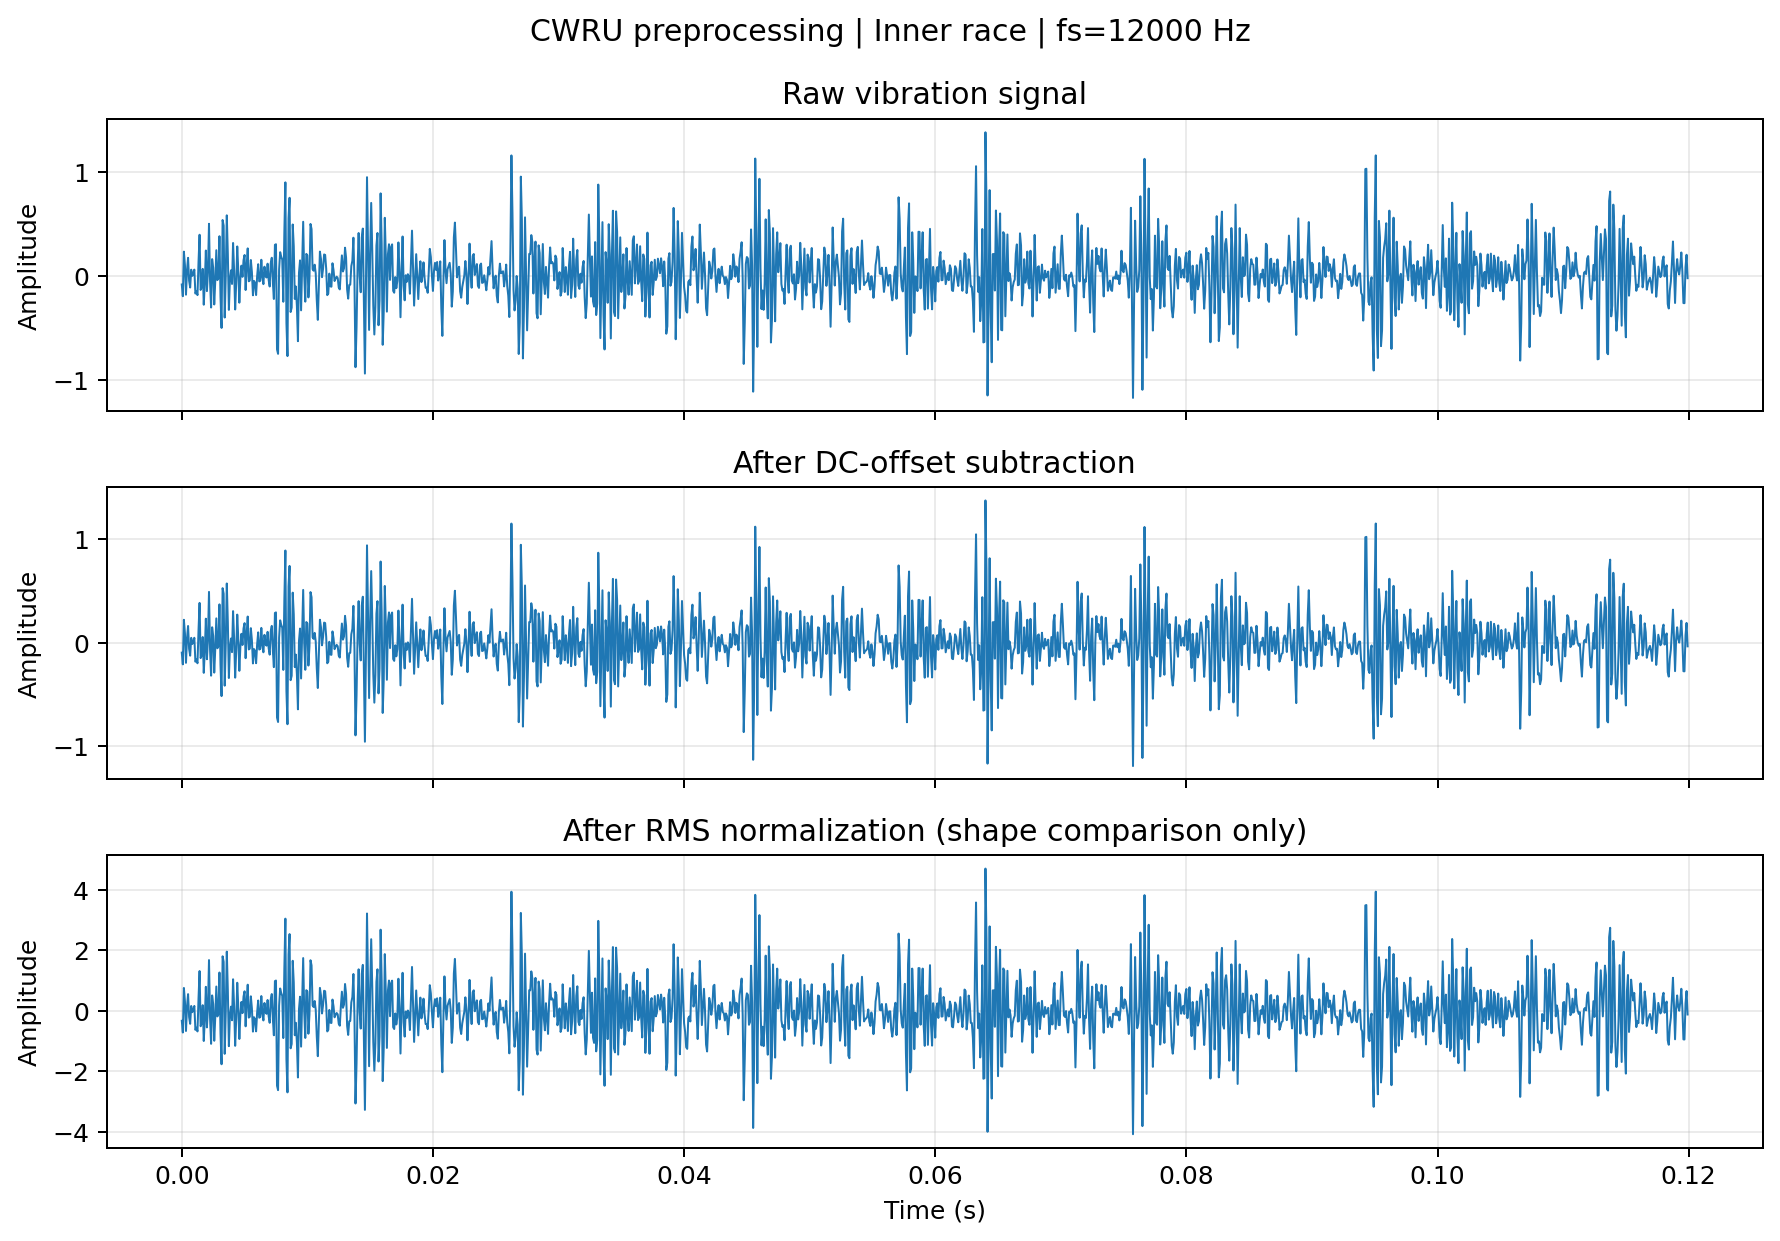
\includegraphics[width=0.60\columnwidth]{figures/figure_1.png}
\captionof{figure}{CWRU inner-race fault: time-domain preprocessing (raw,
DC-removed and RMS-normalized signals).}
\label{fig:m1a1}
\end{minipage}
\end{center}
\vspace{2pt}

\begin{center}
\begin{minipage}{\columnwidth}
\centering
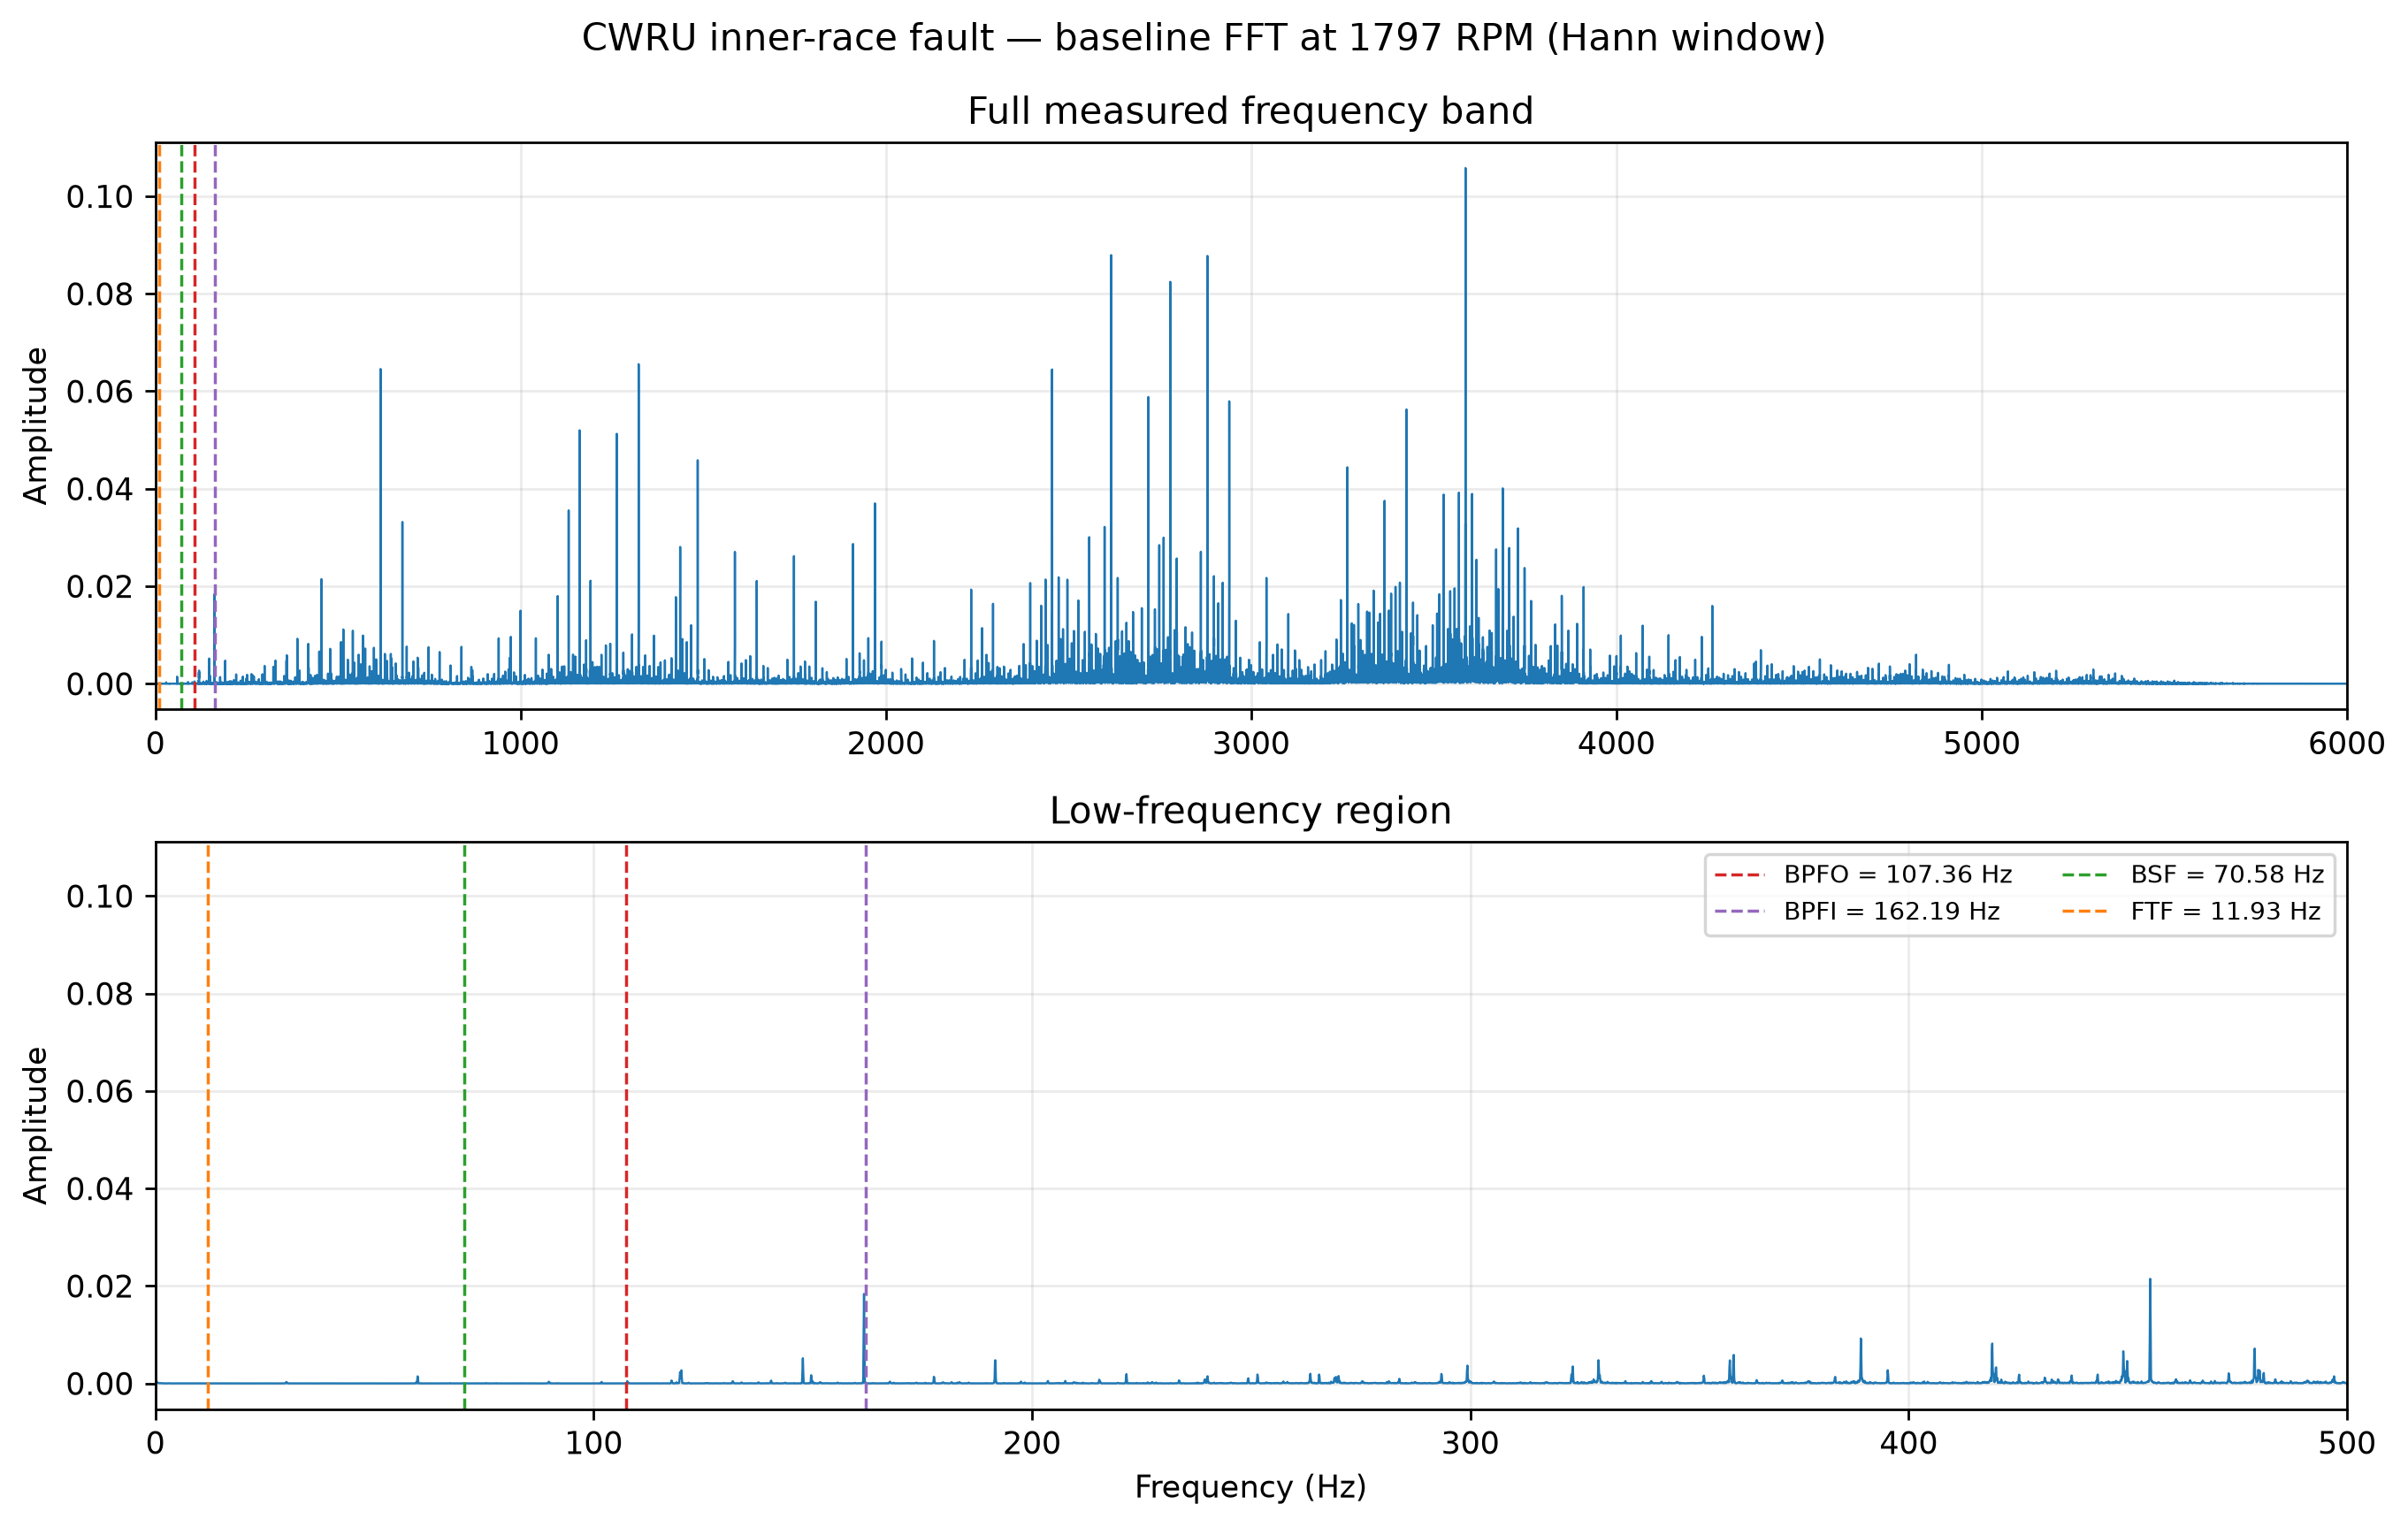
\includegraphics[width=0.60\columnwidth]{figures/figure_2.png}
\captionof{figure}{CWRU inner-race fault: baseline FFT spectrum at
$1797$~rpm.}
\label{fig:m1a2}
\end{minipage}
\end{center}
\vspace{2pt}

\begin{center}
\begin{minipage}{\columnwidth}
\centering
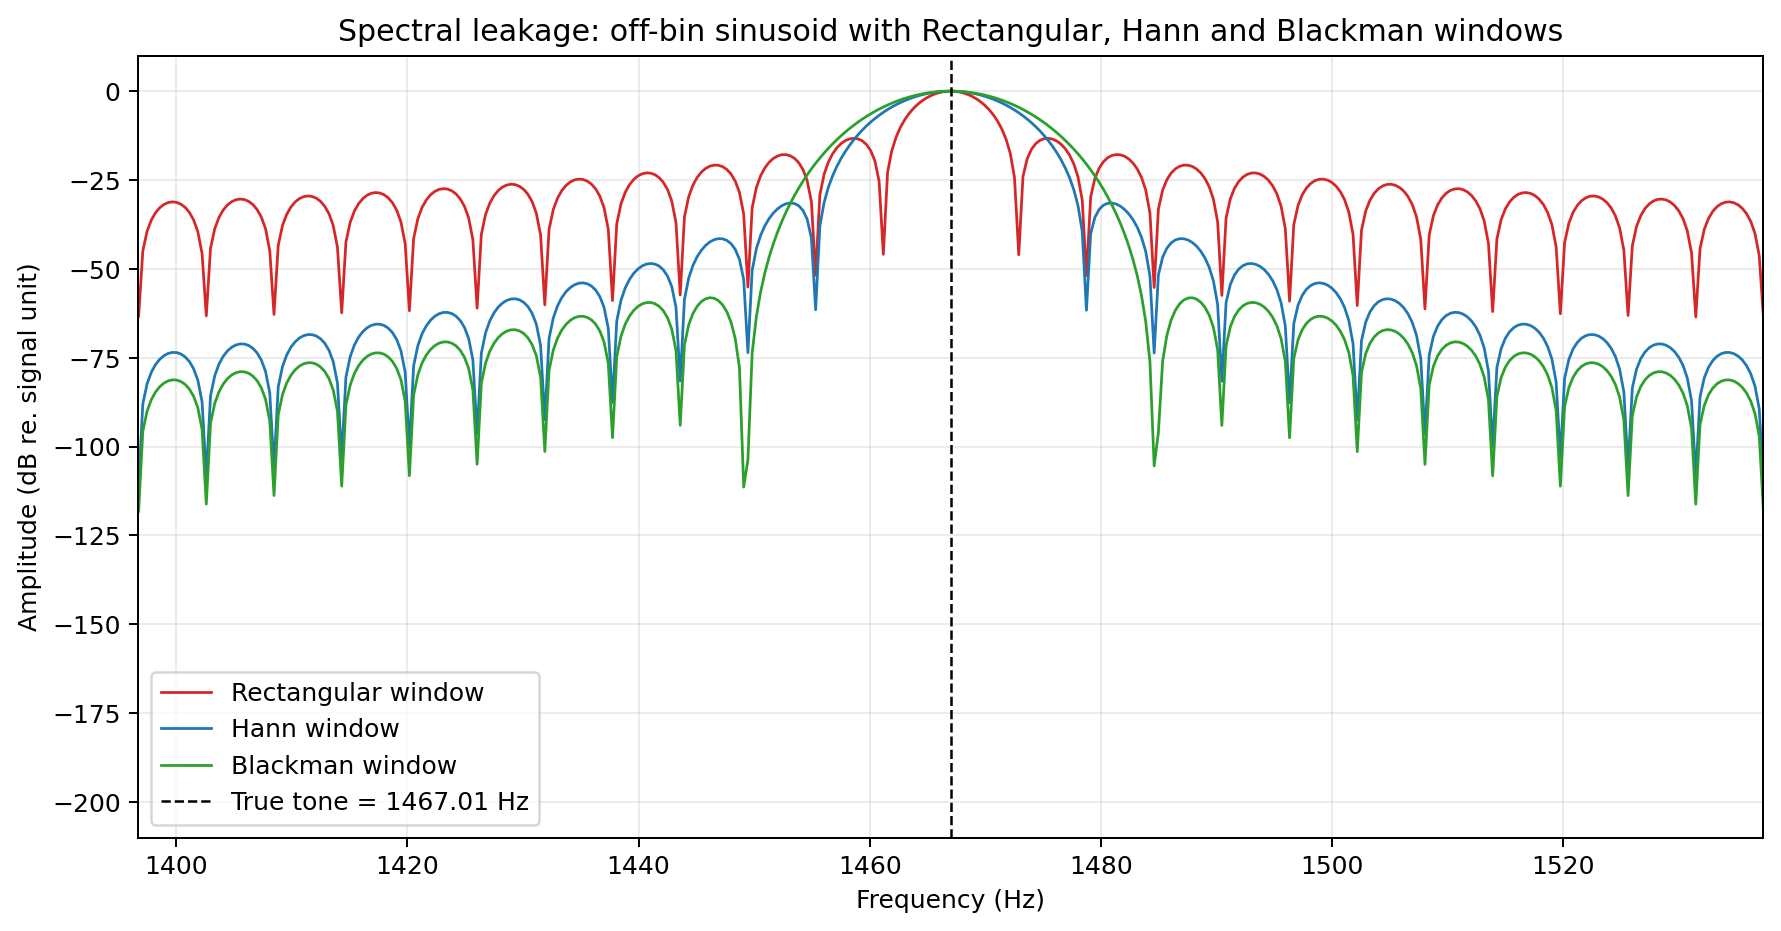
\includegraphics[width=0.60\columnwidth]{figures/figure_3.png}
\captionof{figure}{Controlled off-bin single-tone comparison of the
rectangular, Hann and Blackman windows.}
\label{fig:m1a3}
\end{minipage}
\end{center}
\vspace{2pt}

\begin{center}
\begin{minipage}{\columnwidth}
\centering
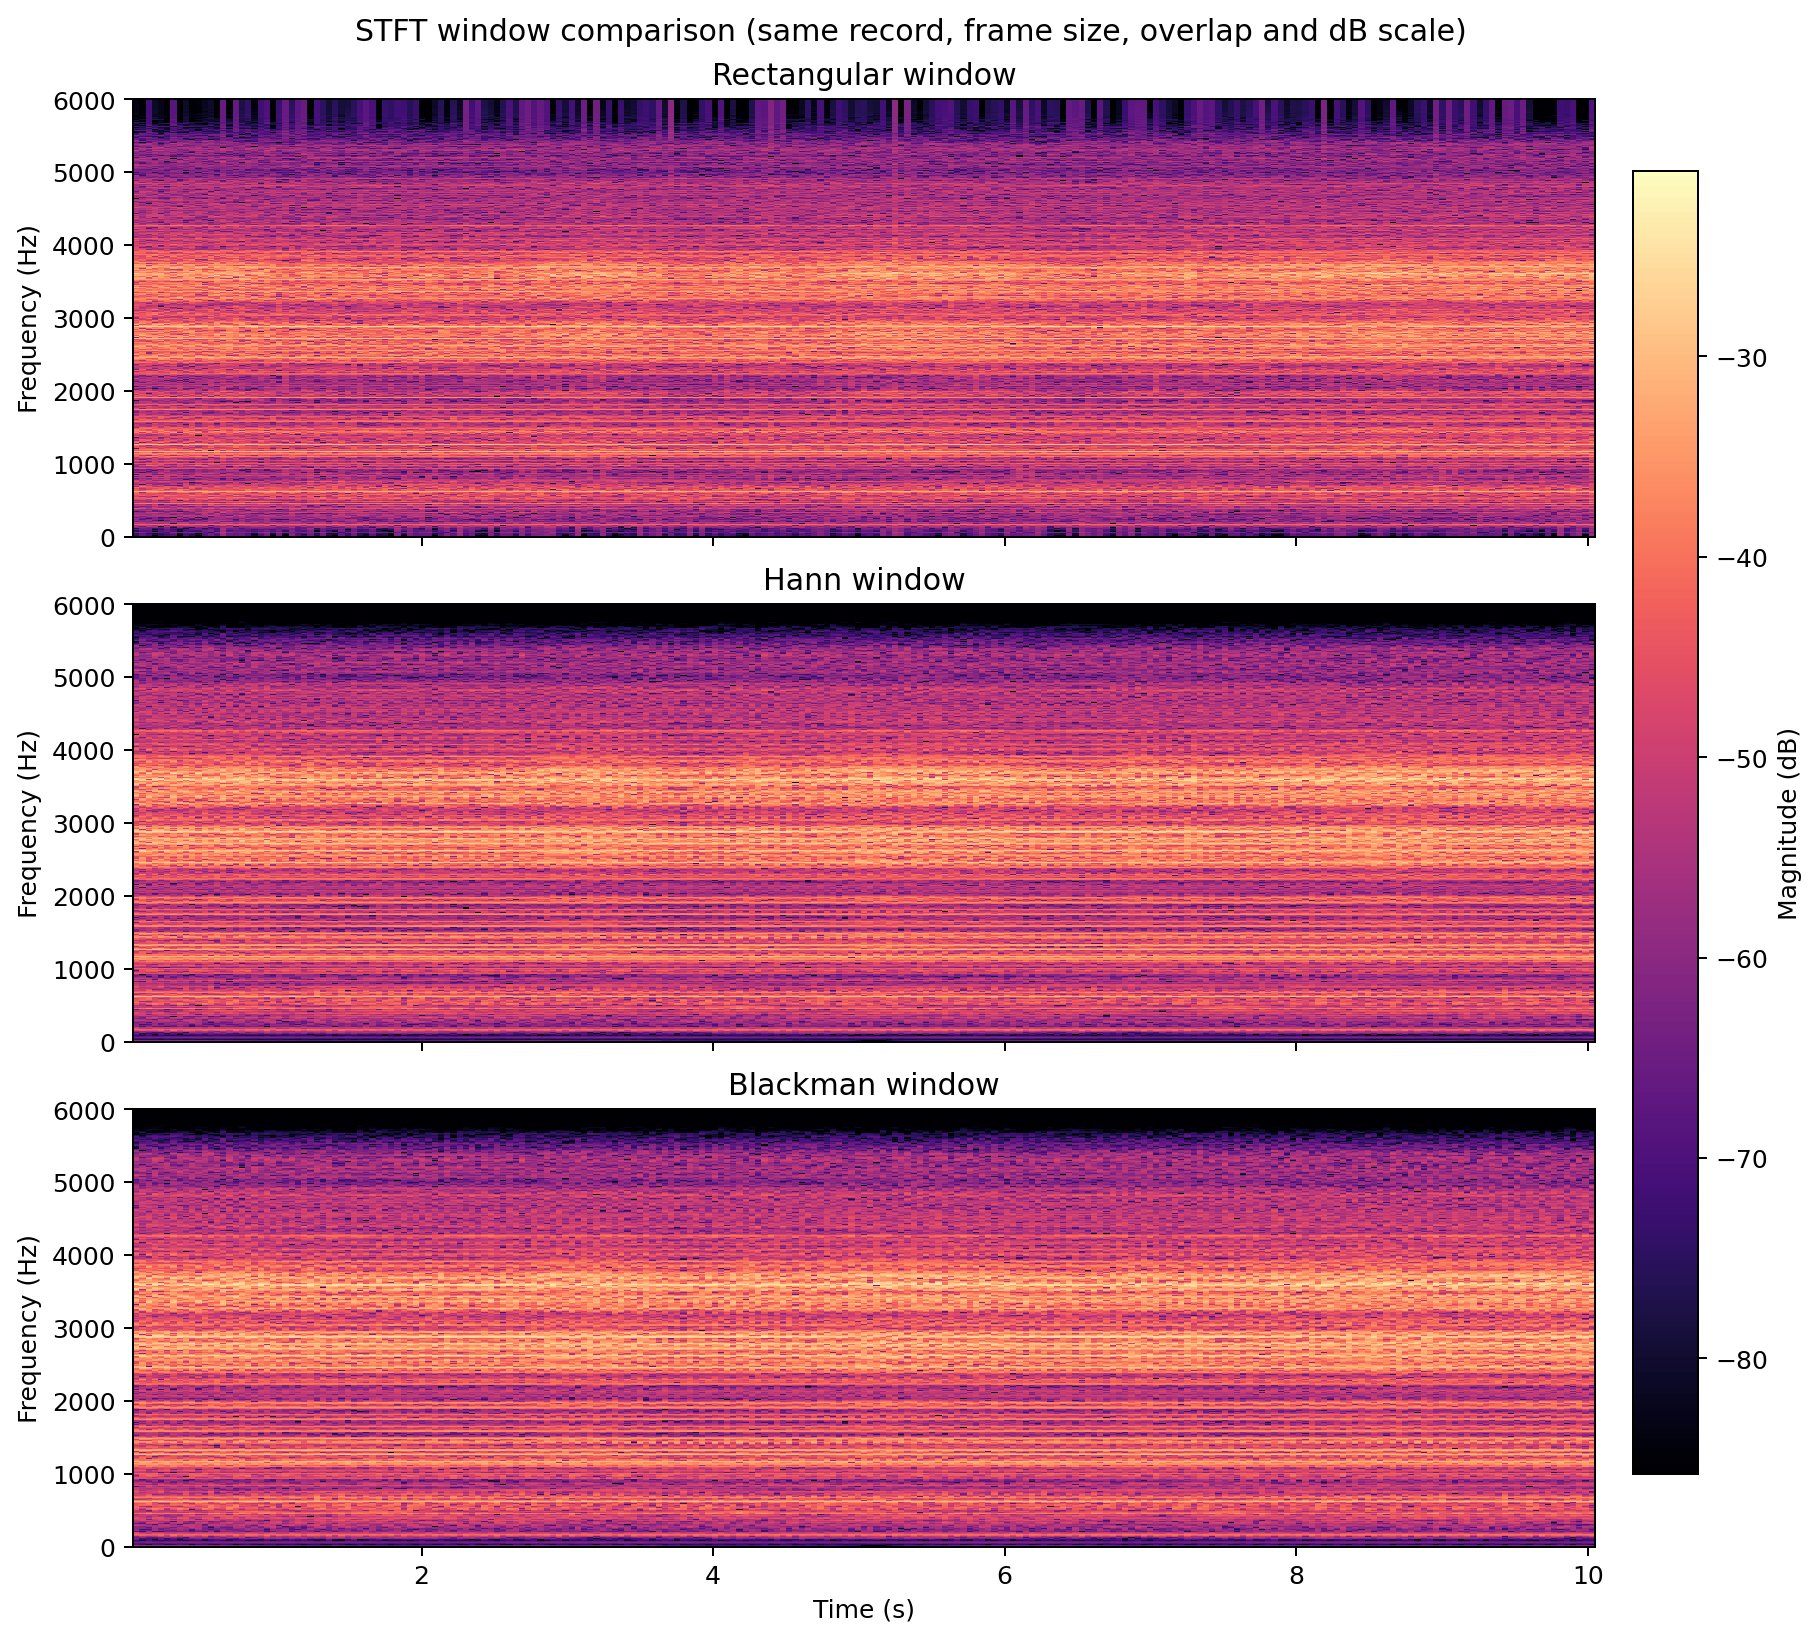
\includegraphics[width=0.60\columnwidth]{figures/figure_4.png}
\captionof{figure}{CWRU inner-race fault: STFT comparison using the
rectangular, Hann and Blackman windows.}
\label{fig:m1a4}
\end{minipage}
\end{center}
\vspace{2pt}

\section{MFPT Baseline Records}
The second set follows the MFPT bearing through its load sweep, before and
after the resonance band is selected.

\begin{center}
\begin{minipage}{\columnwidth}
\centering
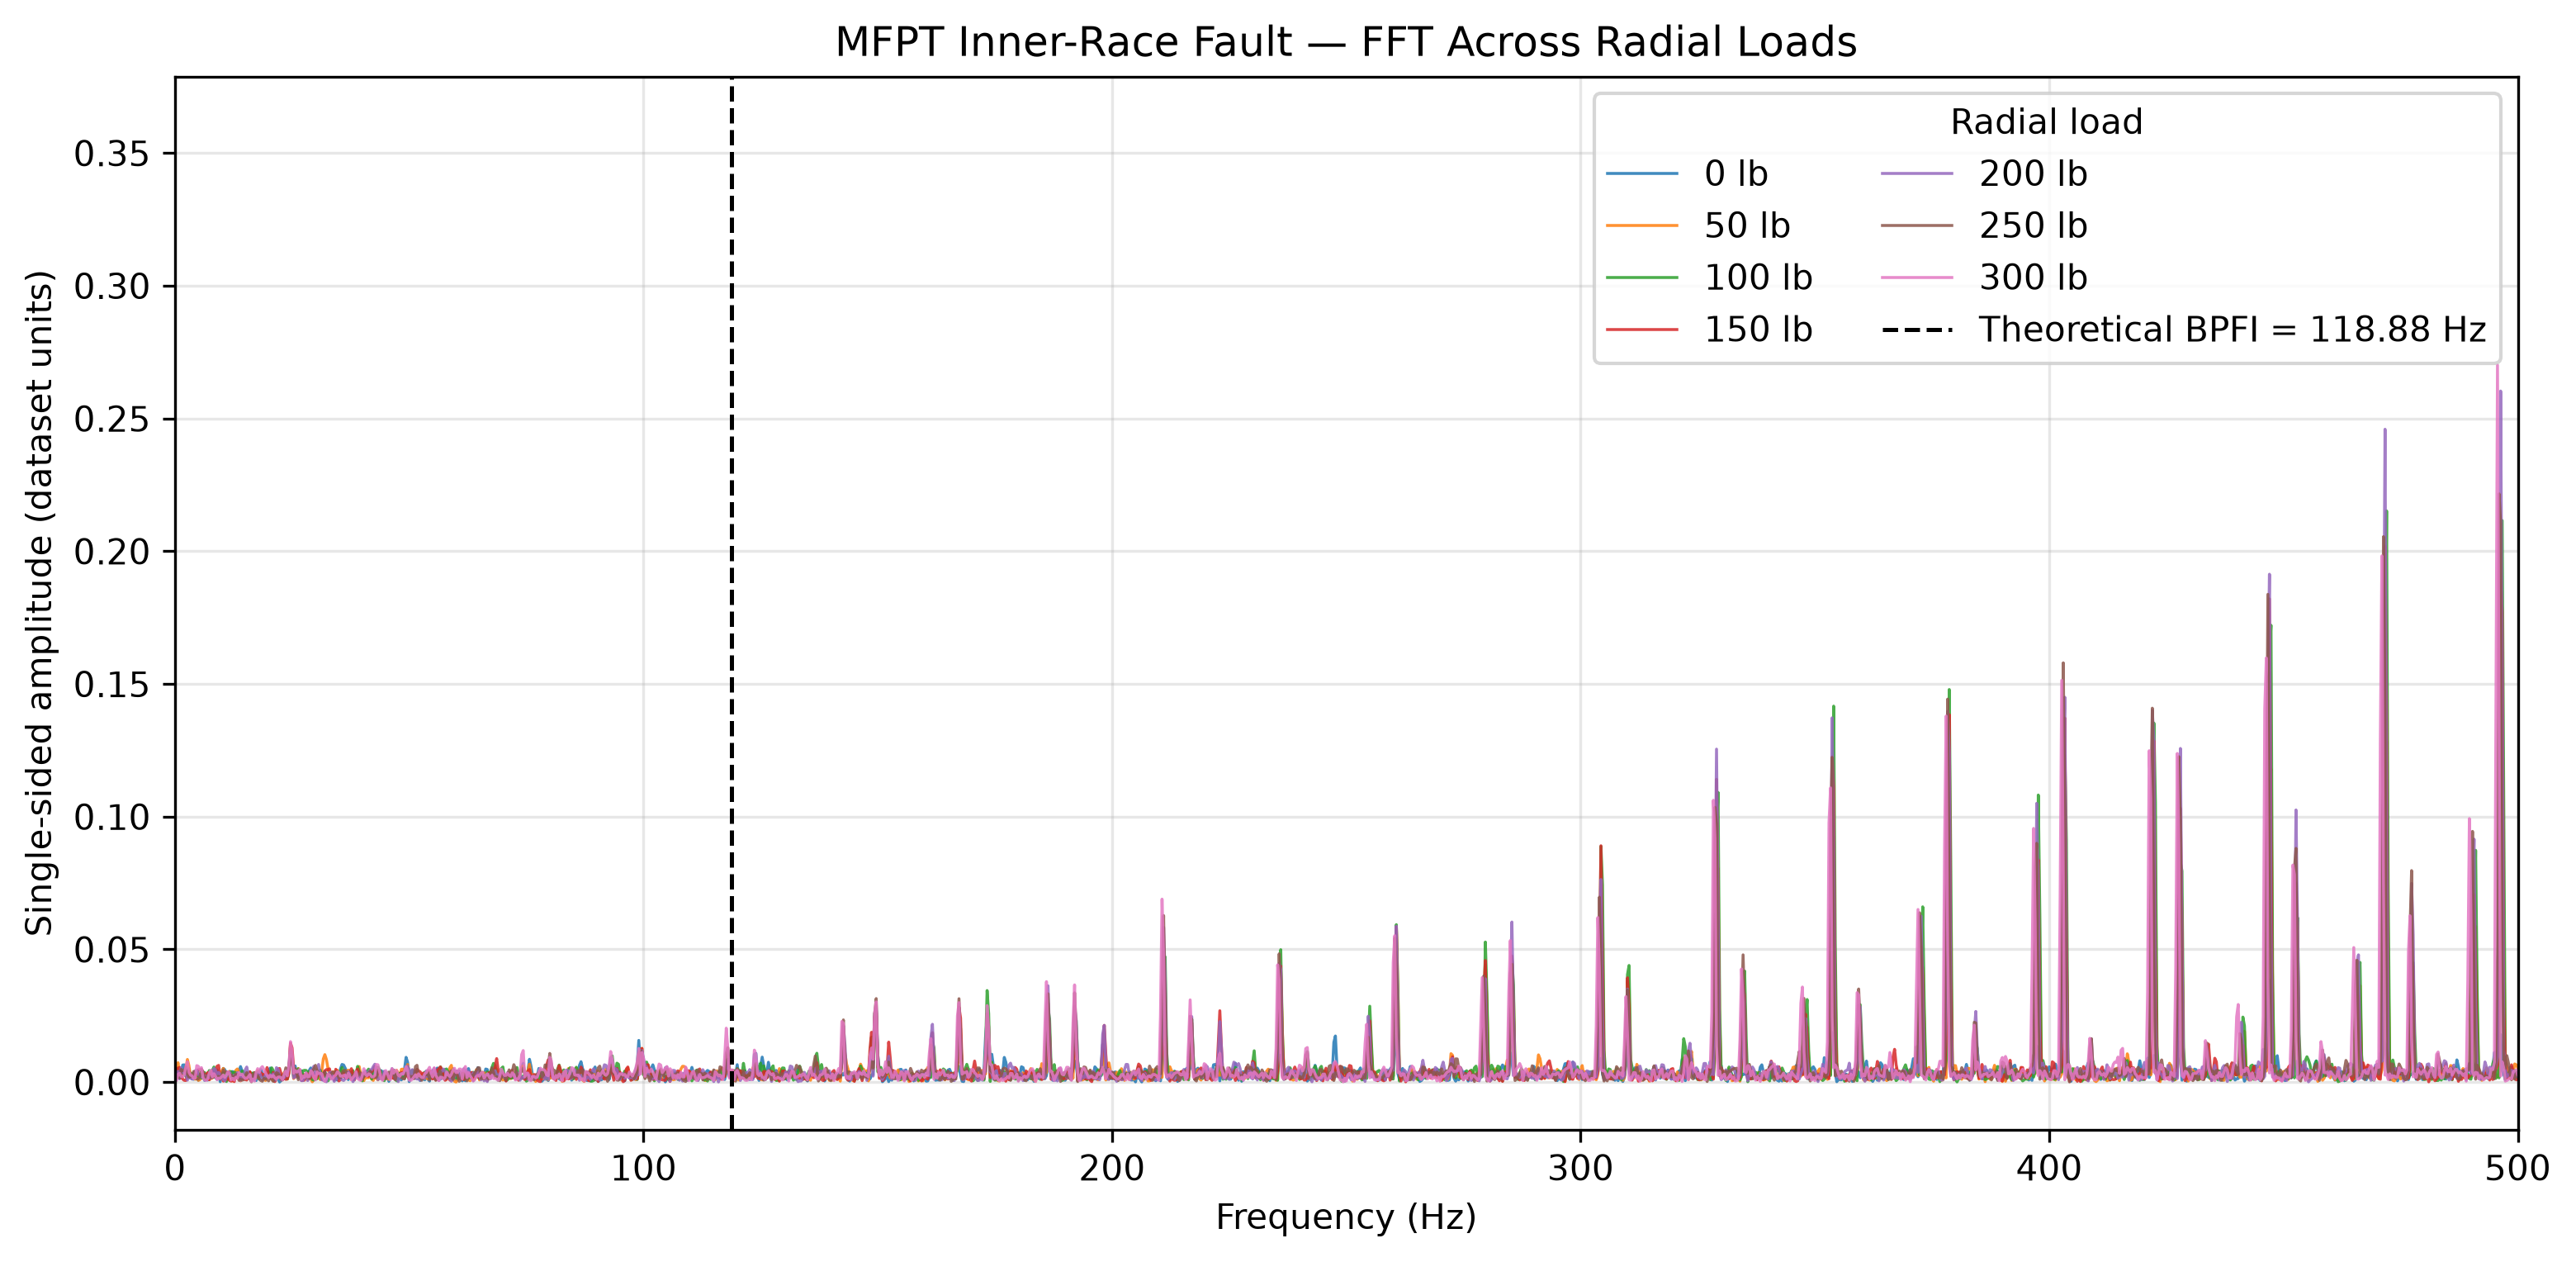
\includegraphics[width=0.60\columnwidth]{figures/figure_5.png}
\captionof{figure}{MFPT inner-race fault: FFT across radial loads.}
\label{fig:m1b1}
\end{minipage}
\end{center}
\vspace{2pt}

\begin{center}
\begin{minipage}{\columnwidth}
\centering
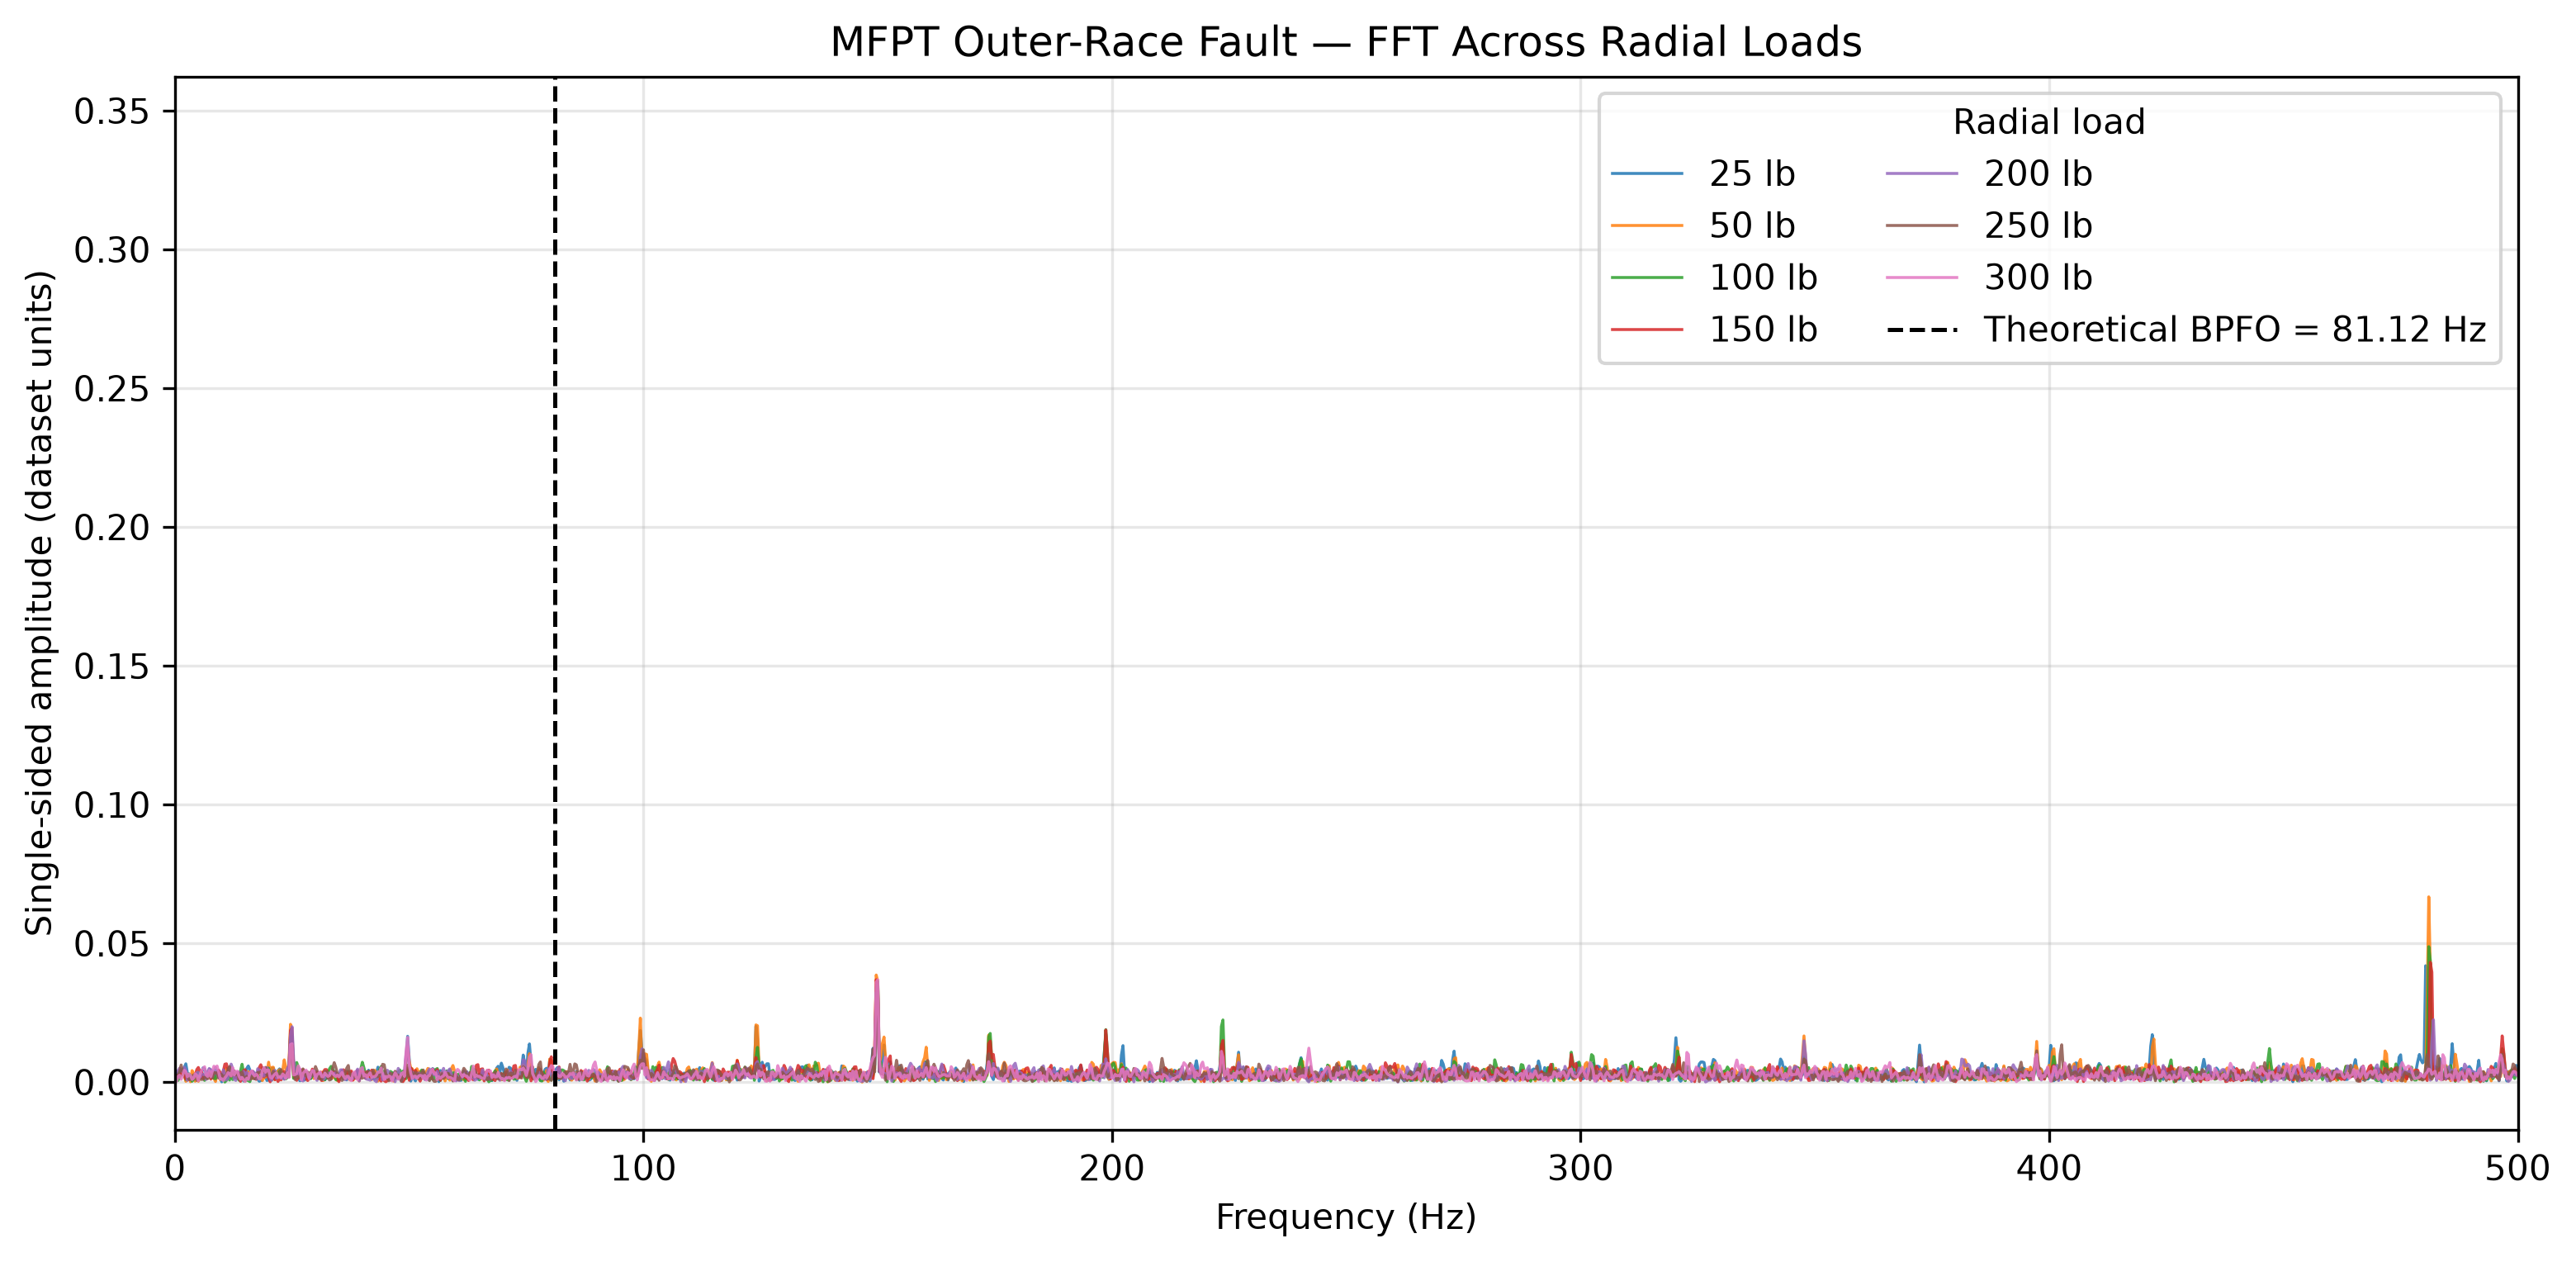
\includegraphics[width=0.60\columnwidth]{figures/figure_6.png}
\captionof{figure}{MFPT outer-race fault: FFT across radial loads.}
\label{fig:m1b2}
\end{minipage}
\end{center}
\vspace{2pt}

\begin{center}
\begin{minipage}{\columnwidth}
\centering
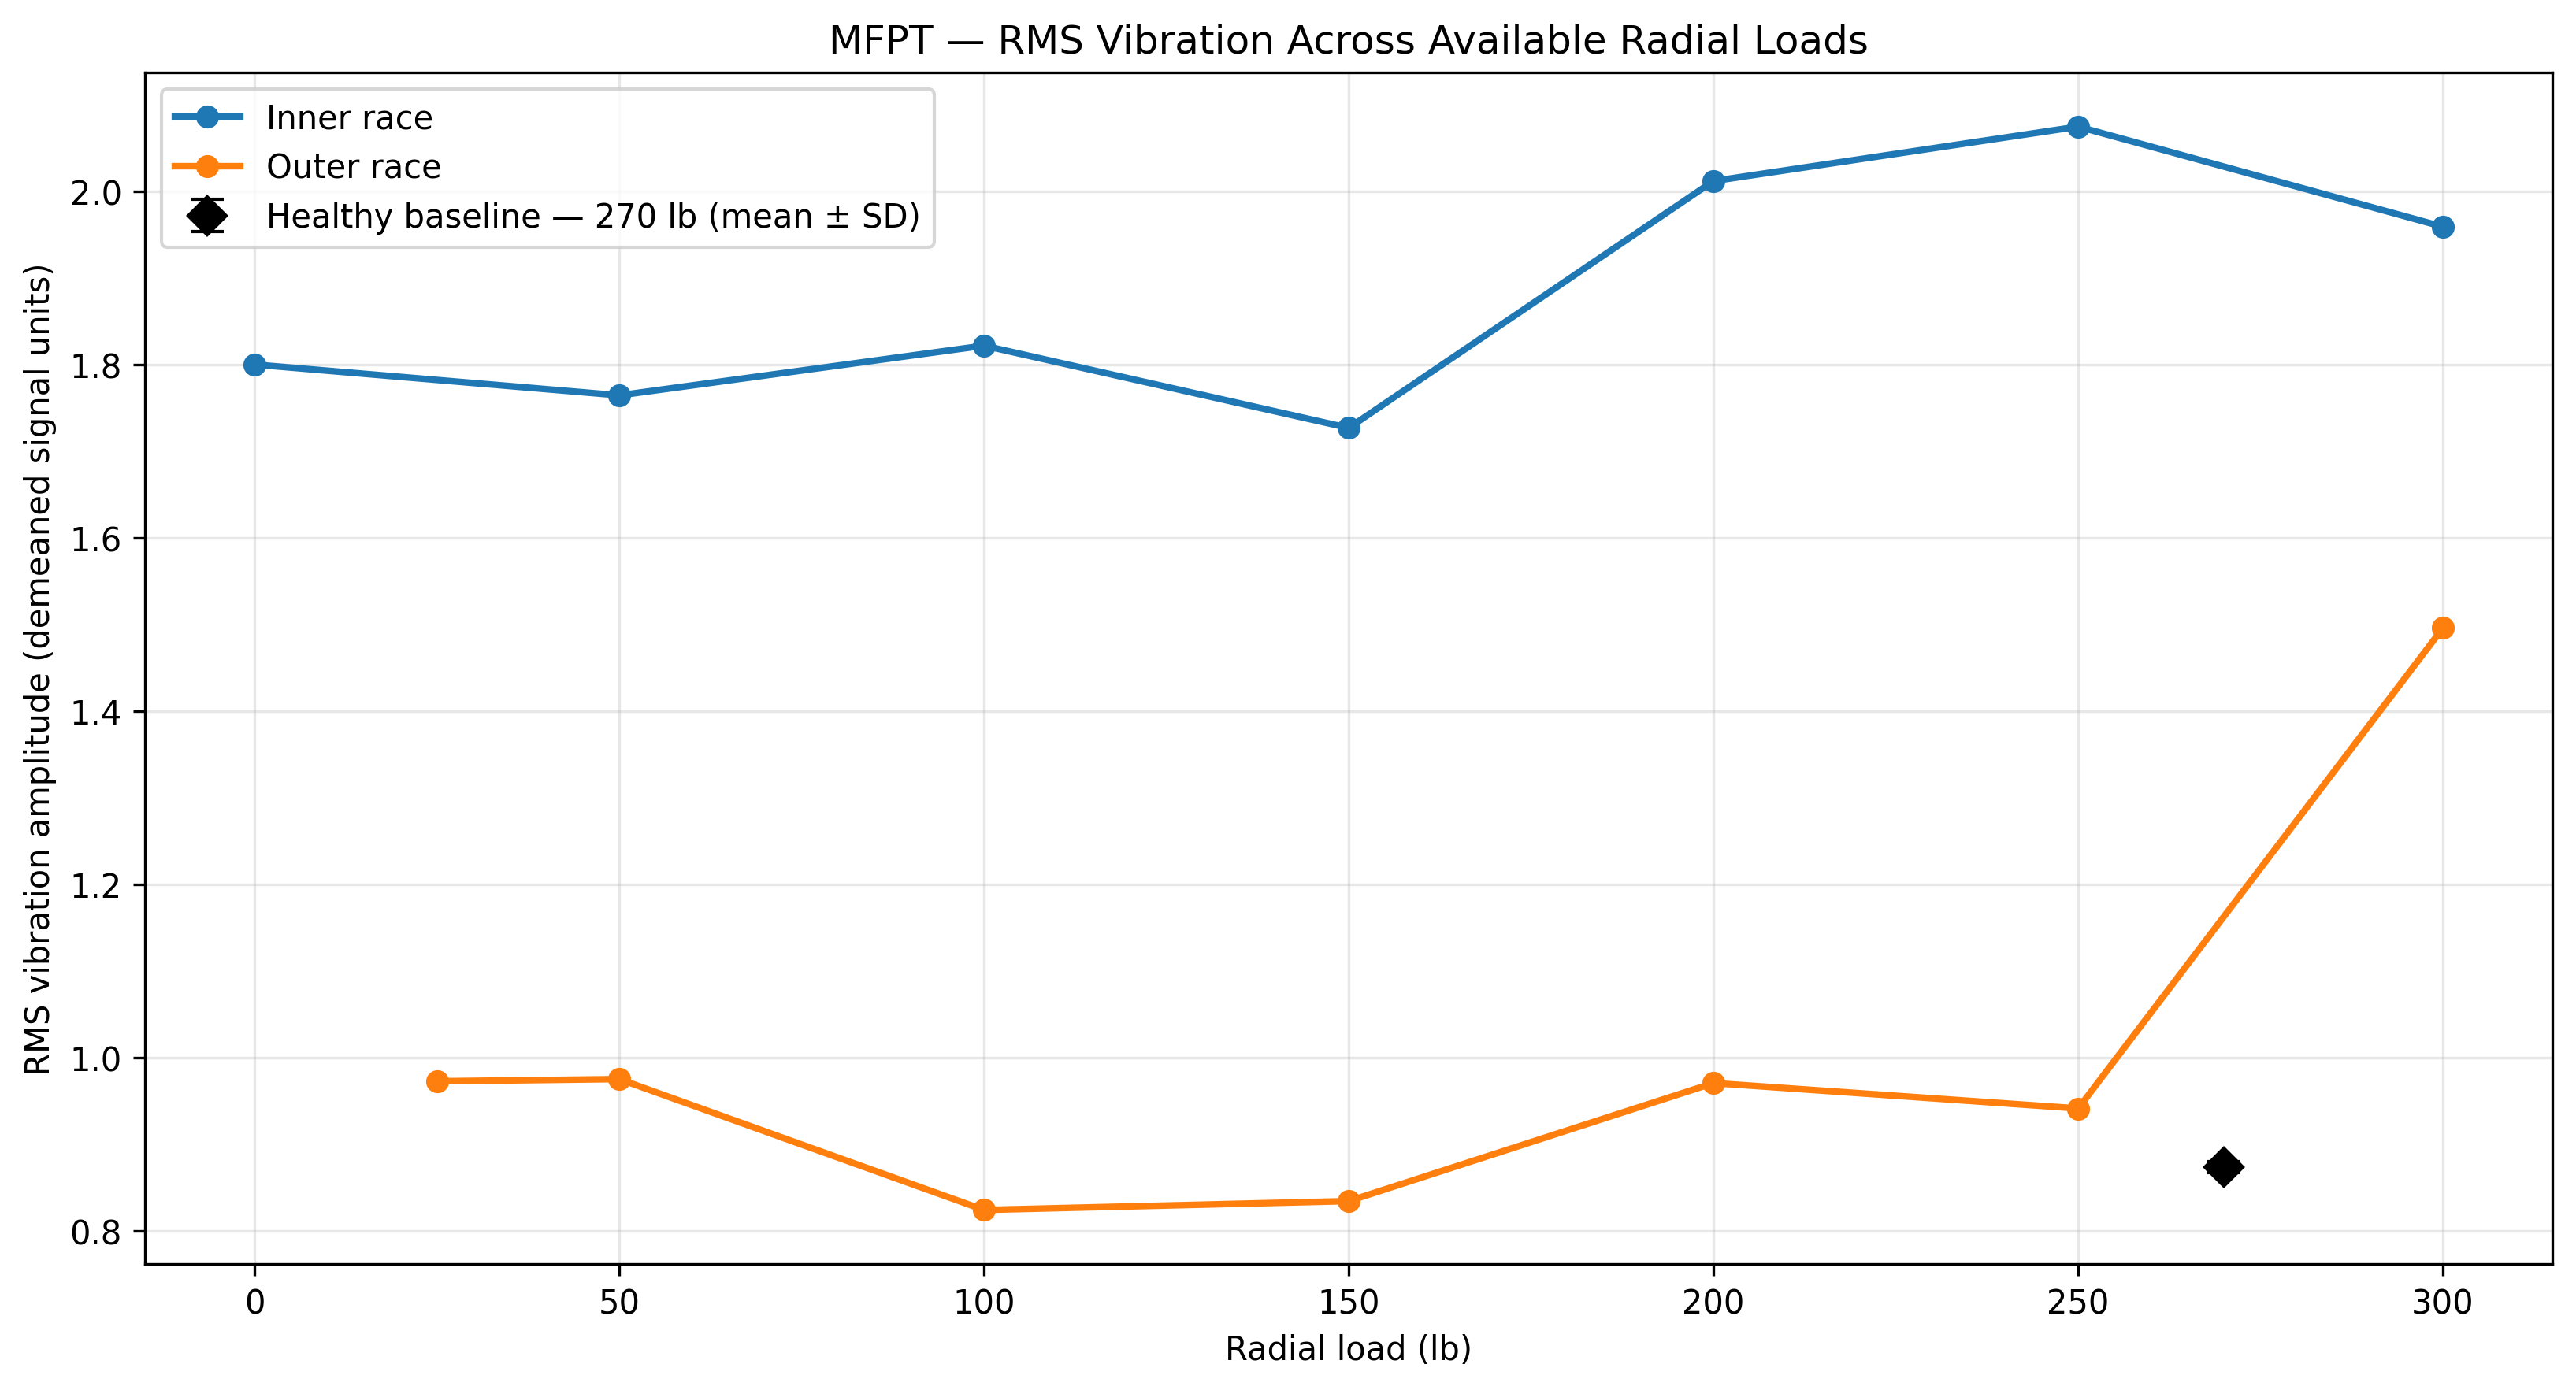
\includegraphics[width=0.60\columnwidth]{figures/figure_7.png}
\captionof{figure}{MFPT RMS vibration amplitude across radial loads.}
\label{fig:m1b3}
\end{minipage}
\end{center}
